%!TEX root = paper.tex
%===================================================================%
% Synthetic data info
%===================================================================%
\newcommand{\calI}{\xmath{\mathcal{I}}}
\newcommand{\calK}{\xmath{\mathcal{K}}}
\newcommand{\calC}{\xmath{\mathcal{C}}}
\newcommand{\calE}{\xmath{\mathcal{E}}}
\newcommand{\calN}{\xmath{\mathcal{N}}}
To assess the validity of our method, we ran experiments on synthetic $4$-D functional connectome data.
The data were generated to imitate functional connectomes resulting from a single slice of our grid-based parcellation scheme (see Fig.~\ref{fig:roi,grid,slice}).
Specifically, we selected only the nodes that are present at axial slice $z=18$ in the MNI space; this slice was selected for its substantial $X$ and $Y$ coverage.
Fig.~\ref{subfig:sim,conn,struct,hc} provides a schematic representation of the selected nodes.

\newcommand{\muhat}{\xmath{\hat{\mu}}}
\newcommand{\mutil}{\xmath{\widetilde{\mu}}}
\newcommand{\sighat}{\xmath{\hat{\sigma}}}
\newcommand{\arctanh}{\text{arctanh}}
To mimic the \emph{control vs. patient} binary classification setup, we created two classes of functional connectomes sampled from random normal distributions. 
The mean and the variance for these distributions were assigned using the functional connectomes generated from the real resting state dataset described later in Sec.~\ref{subsec:real,data}.
Specifically, we first took the subject-level functional connectomes corresponding to the $67$ healthy controls in the dataset, and extracted the entries that represent the edges among the nodes at slice $z=18$.
Since there are $66$ nodes within this slice, this gives us $\binom{66}{2}=2145$ edges for each subjects.
Next, we applied Fisher transformation on these edges to map the correlation values to the real line.
For each of these transformed edges, we calculated the inter-subject sample mean and sample variance, which we denote by $\{\muhat(k),\sighat^2(k)\}$ with $k\in[2145]$ indexing the edges.
Finally, a synthetic subject-level ``control class'' connectome is realized by sampling edges individually from a set of random normal distributions having the above mean and variance, and then applying inverse Fisher transformation $\tanh:\reals\to (-1,+1)$ on these sampled edges, \ie,
\[
	\x=\left[
		\tanh\big(x^{(1)}\big),
		\dots,
		\tanh\big(x^{(2145)}\big)
	\right]^T
	\text{ where } x^{(k)}\sim\calN\left(\muhat(k),\sighat^2(k)\right),\; k\in[2145].
\]
Realizations of the ``patient class'' connectomes are generated in a similar manner, but here we introduced two clusters of \emph{anomalous nodes}, indicated by the red nodes in Fig.~\ref{subfig:sim,conn,struct,ds}.
These clusters participate in a disease-specific perturbation, where signal was added to all connections originating in one cluster and terminating in the other.
More formally, let $\calK\subset[2145]$ denote the index set corresponding to these disease-specific \emph{anomalous edges}, which consist of a complete bipartite graph formed by the anomalous node clusters $\calC_1=\{8,14,15,16,23\}$ and $\calC_2=\{41,48,49,50,56\}$, $\calC_1,\calC_2\subset[66]$.
Under these notations, a synthetic subject-level ``patient class'' connectome is realized by the following procedure:
\[
	\x=\left[
		\tanh\big(x^{(1)}\big),
		\dots,
		\tanh\big(x^{(2145)}\big)
	\right]^T 
	\text{where } 
	\begin{cases}
		x^{(k)}\sim\calN\Big(\muhat(k),\sighat^2(k)\Big) &\text{ if } k\notin\calK \vspace{3pt}\\
		x^{(k)}\sim\calN\Big(\muhat(k)+d\cdot\sighat(k),\;\sighat^2(k)\Big) &\text{ if } k\in\calK\;.
	\end{cases}
\]
In other words, if an edge $k$ is a member of the anomalous edge set \calK, a non-random signal $d\cdot\sighat(k)$ is added to the sampled edge-value.
Here, $d$ denotes Cohen's effect size \citep{Cohen:1988}, which we set at $d=0.6$ for our experiments.
Overall, since $\abs{\calC_1}=\abs{\calC_2}=5$, we have $\abs{\calK}=\abs{\calC_1}\cdot\abs{\calC_2}=25$, \ie, there are $25$ anomalous edges in the patient group; see Fig.~\ref{subfig:sim,conn,struct,ds} for a pictorial illustration of the anomalous edge set \calK in the $2$-D node space.
Fig.~\ref{subfig:sim,conn,struct,supp} presents a binary support matrix indicating the structure of the anomalous edges in the $4$-D connectome space, with the locations of the anomalous edges specified by the product set $\calC_1\times \calC_2\subset[66]\times[66]$. 

%************************ Tikz fig ******************************%
\begin{figure}
	\centering
	\begin{subfigure}[b]{0.25\linewidth}
		 \centering
		 \resizebox{0.94\linewidth}{!}{%!TEX root = paper.tex
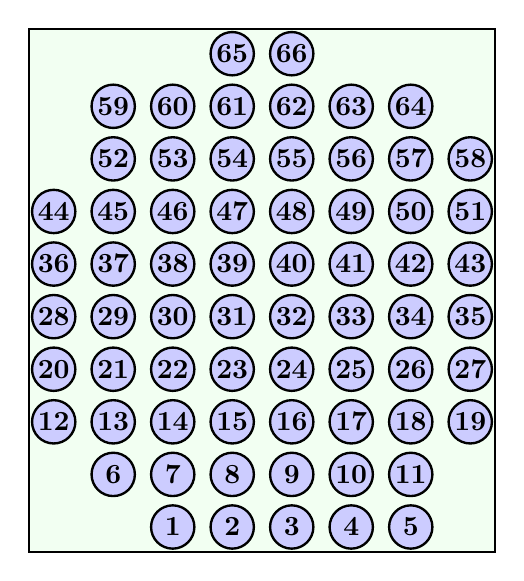
\begin{tikzpicture}[-,red, line width=0.06cm,font=\bfseries,draw=black] 
	\tikzstyle{every node}=[circle,ultra thick,draw=black,fill=white,text=black,minimum size=0.55cm,line width=0.03cm,inner sep=0.8pt]
	\tikzstyle{HC} =[fill=blue!20] % HC = healthy control node
	\tikzstyle{DS} =[fill=blue!20]  % DS = disease node
	\matrix [rectangle,row sep=2.5pt, column sep=5pt,draw=black,fill=green!5,line width=0.025cm] % 
	{
				    ;&				;&				 ;& \node(65)[HC]{65} ;& \node(66)[HC]{66} ;\\
		 		    ;& \node(59)[HC]{59} ;& \node(60)[HC]{60} ;& \node(61)[HC]{61} ;& \node(62)[HC]{62} ;& \node(63)[HC]{63} ;& \node(64)[HC]{64} ;& ;\\
		 		    ;& \node(52)[HC]{52} ;& \node(53)[HC]{53} ;& \node(54)[HC]{54} ;& \node(55)[HC]{55} ;& \node(56)[DS]{56} ;& \node(57)[HC]{57} ;& \node(58)[HC]{58} ;\\
	 \node(44)[HC]{44} ;& \node(45)[HC]{45} ;& \node(46)[HC]{46} ;& \node(47)[HC]{47} ;& \node(48)[DS]{48} ;& \node(49)[DS]{49} ;& \node(50)[DS]{50} ;& \node(51)[HC]{51} ;\\
	 \node(36)[HC]{36} ;& \node(37)[HC]{37} ;& \node(38)[HC]{38} ;& \node(39)[HC]{39} ;& \node(40)[HC]{40} ;& \node(41)[DS]{41} ;& \node(42)[HC]{42} ;& \node(43)[HC]{43} ;\\
	 \node(28)[HC]{28} ;& \node(29)[HC]{29} ;& \node(30)[HC]{30} ;& \node(31)[HC]{31} ;& \node(32)[HC]{32} ;& \node(33)[HC]{33} ;& \node(34)[HC]{34} ;& \node(35)[HC]{35} ;\\
	 \node(20)[HC]{20} ;& \node(21)[HC]{21} ;& \node(22)[HC]{22} ;& \node(23)[DS]{23} ;& \node(24)[HC]{24} ;& \node(25)[HC]{25} ;& \node(26)[HC]{26} ;& \node(27)[HC]{27} ;\\
	 \node(12)[HC]{12} ;& \node(13)[HC]{13} ;& \node(14)[DS]{14} ;& \node(15)[DS]{15} ;& \node(16)[DS]{16} ;& \node(17)[HC]{17} ;& \node(18)[HC]{18} ;& \node(19)[HC]{19} ;\\
		 		    ;& \node(6)[HC]{6} 	;& \node(7)[HC]{7} 	 ;& \node(8)[DS]{8}	  ;& \node(9)[HC]{9}   ;& \node(10)[HC]{10} ;& \node(11)[HC]{11} ;&  ;\\
	 			    ;&				;& \node(1)[HC]{1} 	 ;& \node(2)[HC]{2}	  ;& \node(3)[HC]{3}   ;& \node(4)[HC]{4}   ;& \node(1)[HC]{5}   ;&  ;\\
	};
\end{tikzpicture}
}
		 \caption{Control}
		 \label{subfig:sim,conn,struct,hc}
	\end{subfigure}
	\hspace{-4pt}
	\begin{subfigure}[b]{0.5\linewidth}
		 \centering
		 \resizebox{0.94\linewidth}{!}{%!TEX root = paper.tex
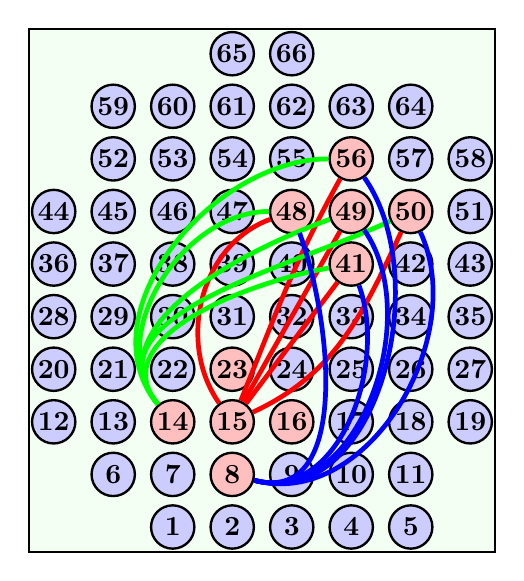
\begin{tikzpicture}[-,red, line width=0.06cm,font=\bfseries,draw=black] 
	\tikzstyle{every node}=[circle,ultra thick,draw=black,fill=white,text=black,minimum size=0.55cm,line width=0.03cm,inner sep=0.8pt]
	\tikzstyle{HC} =[fill=blue!20] % HC = healthy control node
	\tikzstyle{DS} =[fill=red!25]  % DS = disease node
	\matrix [rectangle,row sep=2.5pt, column sep=5pt,draw=black,fill=green!5,line width=0.025cm] % 
	{
				    ;&				;&				 ;& \node(65)[HC]{65} ;& \node(66)[HC]{66} ;\\
		 		    ;& \node(59)[HC]{59} ;& \node(60)[HC]{60} ;& \node(61)[HC]{61} ;& \node(62)[HC]{62} ;& \node(63)[HC]{63} ;& \node(64)[HC]{64} ;& ;\\
		 		    ;& \node(52)[HC]{52} ;& \node(53)[HC]{53} ;& \node(54)[HC]{54} ;& \node(55)[HC]{55} ;& \node(56)[DS]{56} ;& \node(57)[HC]{57} ;& \node(58)[HC]{58} ;\\
	 \node(44)[HC]{44} ;& \node(45)[HC]{45} ;& \node(46)[HC]{46} ;& \node(47)[HC]{47} ;& \node(48)[DS]{48} ;& \node(49)[DS]{49} ;& \node(50)[DS]{50} ;& \node(51)[HC]{51} ;\\
	 \node(36)[HC]{36} ;& \node(37)[HC]{37} ;& \node(38)[HC]{38} ;& \node(39)[HC]{39} ;& \node(40)[HC]{40} ;& \node(41)[DS]{41} ;& \node(42)[HC]{42} ;& \node(43)[HC]{43} ;\\
	 \node(28)[HC]{28} ;& \node(29)[HC]{29} ;& \node(30)[HC]{30} ;& \node(31)[HC]{31} ;& \node(32)[HC]{32} ;& \node(33)[HC]{33} ;& \node(34)[HC]{34} ;& \node(35)[HC]{35} ;\\
	 \node(20)[HC]{20} ;& \node(21)[HC]{21} ;& \node(22)[HC]{22} ;& \node(23)[DS]{23} ;& \node(24)[HC]{24} ;& \node(25)[HC]{25} ;& \node(26)[HC]{26} ;& \node(27)[HC]{27} ;\\
	 \node(12)[HC]{12} ;& \node(13)[HC]{13} ;& \node(14)[DS]{14} ;& \node(15)[DS]{15} ;& \node(16)[DS]{16} ;& \node(17)[HC]{17} ;& \node(18)[HC]{18} ;& \node(19)[HC]{19} ;\\
		 		    ;& \node(6)[HC]{6} 	;& \node(7)[HC]{7} 	 ;& \node(8)[DS]{8}	  ;& \node(9)[HC]{9}   ;& \node(10)[HC]{10} ;& \node(11)[HC]{11} ;&  ;\\
	 			    ;&				;& \node(1)[HC]{1} 	 ;& \node(2)[HC]{2}	  ;& \node(3)[HC]{3}   ;& \node(4)[HC]{4}   ;& \node(1)[HC]{5}   ;&  ;\\
	};
	% edge group red
	\tikzstyle{col}=[red] 
	\draw(15)to[](41)[col];
	\draw(15)to[out=125,in=-160](48)[col];
	\draw(15)to[](49)[col];
	\draw(15)to[out=25,in=-115](50)[col];
	\draw(15)to[out=68,in=-119](56)[col];
	% edge group green
	\tikzstyle{col}=[green!100] 
	\draw(14)to[out=130,in=190](41)[col];
	\draw(14)to[out=130,in=180](48)[col];
	\draw(14)to[out=130,in=200](49)[col];
	\draw(14)to[out=130,in=205](50)[col];
	\draw(14)to[out=130,in=180](56)[col];	
	% edge group blue
	\tikzstyle{col}=[blue] 
	\draw(8)to[out=-15,in=-70](41)[col];
	\draw(8)to[out=-15,in=-70](48)[col];
	\draw(8)to[out=-15,in=-55](49)[col];
	\draw(8)to[out=-15,in=-65](50)[col];
	\draw(8)to[out=-15,in=-55](56)[col];
\end{tikzpicture}
\begin{tikzpicture}[-,red, line width=0.06cm,font=\bfseries,draw=black] 
	\tikzstyle{every node}=[circle,ultra thick,draw=black,fill=white,text=black,minimum size=0.55cm,line width=0.03cm,inner sep=0.8pt]
	\tikzstyle{HC} =[fill=blue!20] % HC = healthy control node
	\tikzstyle{DS} =[fill=red!25]  % DS = disease node
	\matrix [rectangle,row sep=2.5pt, column sep=5pt,draw=black,fill=green!5,line width=0.025cm] % 
	{
				    ;&				;&				 ;& \node(65)[HC]{65} ;& \node(66)[HC]{66} ;\\
		 		    ;& \node(59)[HC]{59} ;& \node(60)[HC]{60} ;& \node(61)[HC]{61} ;& \node(62)[HC]{62} ;& \node(63)[HC]{63} ;& \node(64)[HC]{64} ;& ;\\
		 		    ;& \node(52)[HC]{52} ;& \node(53)[HC]{53} ;& \node(54)[HC]{54} ;& \node(55)[HC]{55} ;& \node(56)[DS]{56} ;& \node(57)[HC]{57} ;& \node(58)[HC]{58} ;\\
	 \node(44)[HC]{44} ;& \node(45)[HC]{45} ;& \node(46)[HC]{46} ;& \node(47)[HC]{47} ;& \node(48)[DS]{48} ;& \node(49)[DS]{49} ;& \node(50)[DS]{50} ;& \node(51)[HC]{51} ;\\
	 \node(36)[HC]{36} ;& \node(37)[HC]{37} ;& \node(38)[HC]{38} ;& \node(39)[HC]{39} ;& \node(40)[HC]{40} ;& \node(41)[DS]{41} ;& \node(42)[HC]{42} ;& \node(43)[HC]{43} ;\\
	 \node(28)[HC]{28} ;& \node(29)[HC]{29} ;& \node(30)[HC]{30} ;& \node(31)[HC]{31} ;& \node(32)[HC]{32} ;& \node(33)[HC]{33} ;& \node(34)[HC]{34} ;& \node(35)[HC]{35} ;\\
	 \node(20)[HC]{20} ;& \node(21)[HC]{21} ;& \node(22)[HC]{22} ;& \node(23)[DS]{23} ;& \node(24)[HC]{24} ;& \node(25)[HC]{25} ;& \node(26)[HC]{26} ;& \node(27)[HC]{27} ;\\
	 \node(12)[HC]{12} ;& \node(13)[HC]{13} ;& \node(14)[DS]{14} ;& \node(15)[DS]{15} ;& \node(16)[DS]{16} ;& \node(17)[HC]{17} ;& \node(18)[HC]{18} ;& \node(19)[HC]{19} ;\\
		 		    ;& \node(6)[HC]{6} 	;& \node(7)[HC]{7} 	 ;& \node(8)[DS]{8}	  ;& \node(9)[HC]{9}   ;& \node(10)[HC]{10} ;& \node(11)[HC]{11} ;&  ;\\
	 			    ;&				;& \node(1)[HC]{1} 	 ;& \node(2)[HC]{2}	  ;& \node(3)[HC]{3}   ;& \node(4)[HC]{4}   ;& \node(1)[HC]{5}   ;&  ;\\
	};
	%********************** Style 2 **************************%
%	% edge group red
	\tikzstyle{col}=[black] 
	\draw(23)to[out=15,in=-90](41)[col];
	\draw(23)to[](48)[col];
	\draw(23)to[](49)[col];
	\draw(23)to[out=0,in=-90](50)[col];
	\draw(23)to[out=90,in=180](56)[col];

	% edge group yellow
	\tikzstyle{col}=[myorange] 
	\draw(16)to[in=-80](41)[col];
	\draw(16)to[](48)[col];
	\draw(16)to[out=78,in=-120](49)[col];
	\draw(16)to[out=30,in=-80](50)[col];
	\draw(16)to[out=82,in=-123](56)[col];
\end{tikzpicture}
}
		 \caption{Patient}
		 \label{subfig:sim,conn,struct,ds}
	\end{subfigure}
	\begin{subfigure}[b]{0.235\linewidth}
		 \centering
		 \raisebox{0pt}{\hspace{-8pt}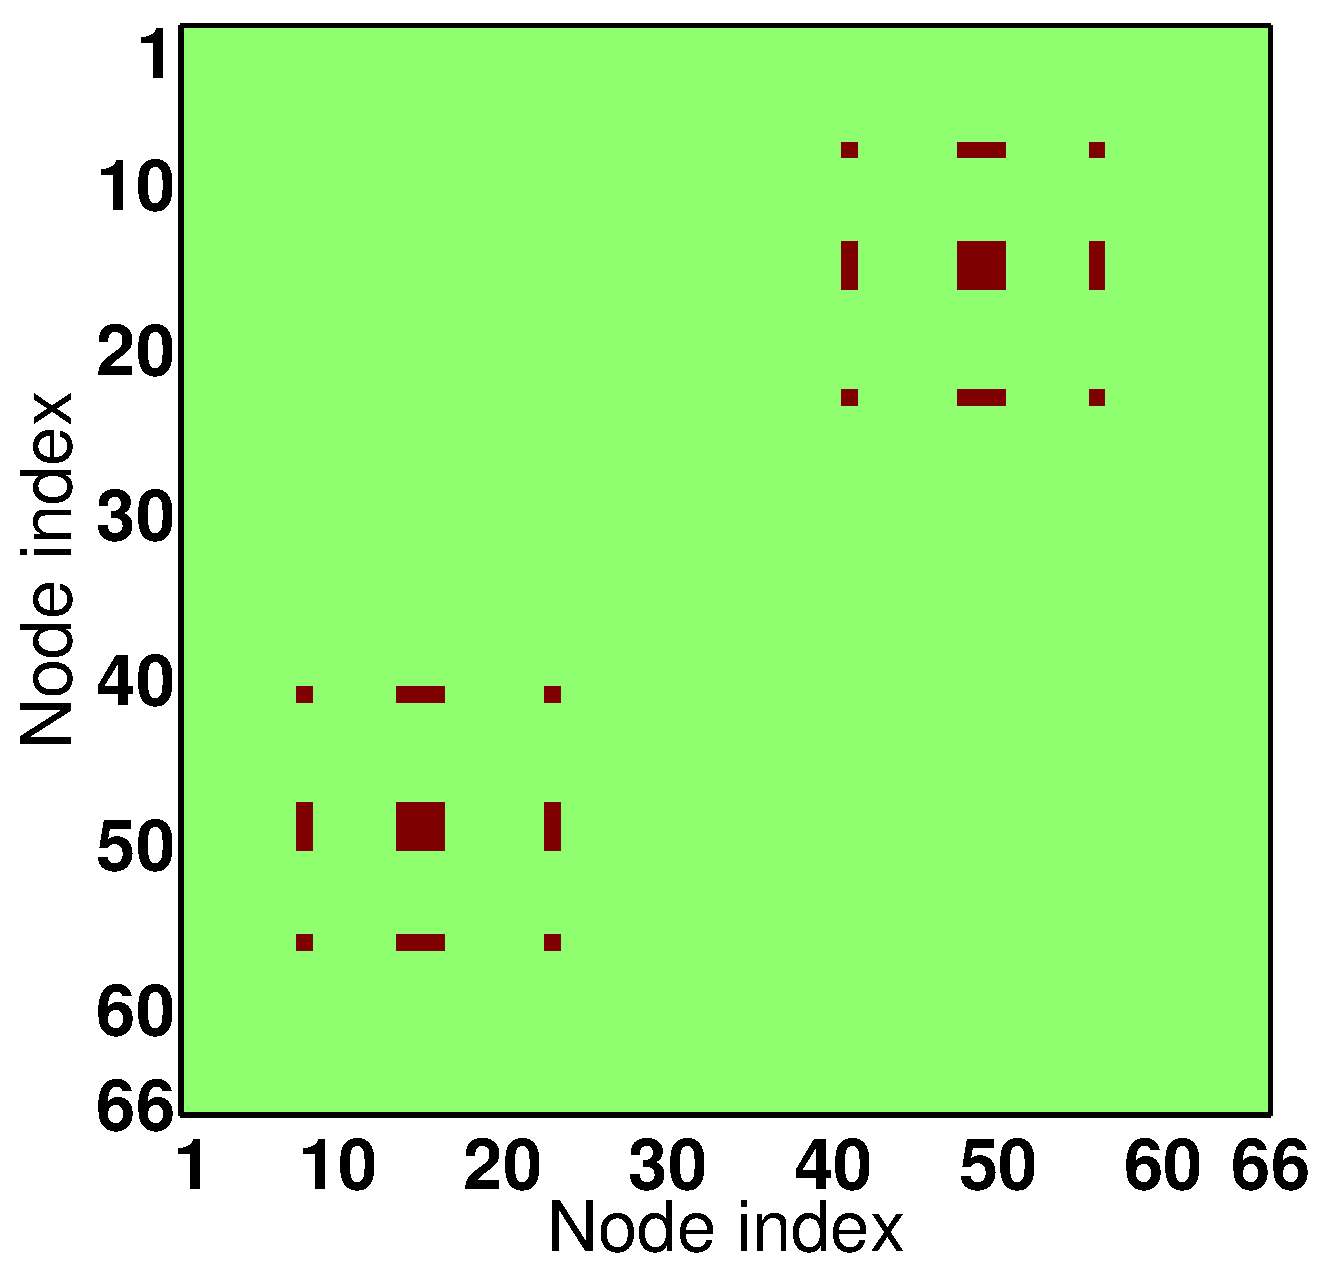
\includegraphics[width=1.125\linewidth]{\fig/sim_weight_truth.pdf}}\vspace{-5pt}\\
		 \caption{Edge support}
		 \label{subfig:sim,conn,struct,supp}
	\end{subfigure}
	\vspace{-12pt}
	\caption{
		Schematic representations of the synthetic $4$-D functional connectome data generated for the simulation experiments (best viewed in color). 
		(a) Node orientation representing the ``control class'' connectome, where the blue nodes indicate
the normal nodes.
		(b) Node orientation representing the ``patient class'' connectome, where there are $25$ \emph{anomalous edges} shared among the two \emph{anomalous node} clusters indicated in red (this subfigure is split into two side-by-side figures to improve visibility of the impacted edges).
		(c) Binary support matrix indicating the locations of the anomalous edges in the connectome space.
	}
	\label{fig:sim,conn,struct}
\end{figure}
%****************************************************************%

It is important to note that the inclusion of the clusters of anomalous nodes is motivated from the ``patchiness assumption'' of brain disorders, a view that has been born from multiple task-based and connectivity-based studies; this point will be expounded in finer detail in \ref{subsec:why,flasso}.
In short, the ``patchiness assumption'' is the view that major psychiatric disorders manifest in the brain by impacting moderately sized spatially contiguous regions,  which is what the clusters of anomalous nodes are intended to mimic in this simulation.

For training the classifiers, we sampled $100$ functional connectomes consisting of $50$ control samples and $50$ patient samples. 
For evaluating the performance of the classifiers, we sampled $500$ additional functional connectomes consisting of $250$ control samples and $250$ patient samples.
